\chapter{The Hardware Architecture of a High-Speed Router}
\label{chap:arch}

This chapter describes the hardware architecture of a high-speed router to
provide the reader with a mental model of a router chip for the rest of this
dissertation. We first describe the main functions of a router. We then
describe the performance requirements for a high-speed router today. Motivated
by these performance requirements, we consider two strawman hardware
architectures and explain their shortcomings. We then describe the predominant
pipeline-based architecture of high-speed routers today. We conclude by
describing how the programmable hardware primitives proposed by this
dissertation fit within the hardware architecture of a high-speed router.

\section{Overview of a router's functionality}
%TODO: Maybe introduce match-action in the previous section?

A router's functionality can be divided into two major planes: the {\em control
plane} and the {\em data plane}. The control plane is responsible for network
management functionality such as running distributed routing protocols (\eg
BGP, IS-IS, and OSPF) to enable end-to-end connectivity, creating access
control rules, and setting up tunnels for network virtualization. The control
plane writes rules into a router's {\em match-action tables}.\footnote{Also
known as lookup tables, routing tables, or just tables.} Each rule in one of
these tables specifies that the router must carry out a specific {\em action}
on a packet if the incoming packet's header {\em matches} a particular pattern.
As an example, a rule could instruct the router to transmit a packet on a
particular output port (action) if the packet has a certain destination IP address
(match).

The data plane is responsible for reading the match-action table and carrying
out the appropriate action operation on every packet.  The data plane matches
the relevant packet headers against the match part of a match-action table
rule. If the packet matches a particular rule, the data plane carries out the
action half of that rule on the packet's headers. If the packet does not match
any rule, some default action is carried out.

The control plane typically runs when the network's topology or the network's
policy changes. The data plane, on the other hand, needs to run on every
packet. The rate of policy or topology changes is typically much less than the
rate at which packets are processed at a router. Hence, the control plane runs
on a general-purpose CPU, while the data plane is implemented in dedicated
hardware as part of a router chip.  Figure~\ref{fig:router_box} shows
an example router with its control and data planes.

\begin{figure}
\centering
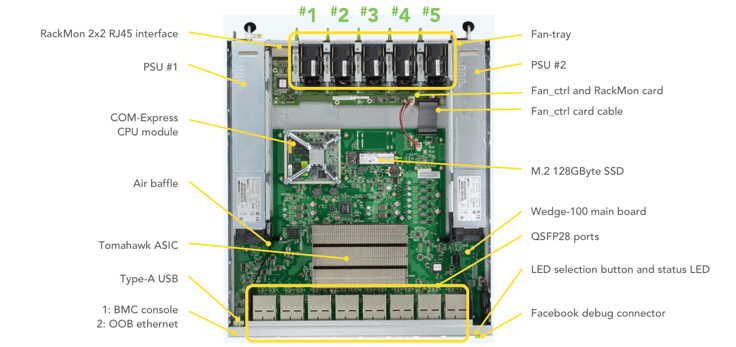
\includegraphics[width=\textwidth]{wedge100.png}
\caption{Facebook's Wedge 100 router from the Open Compute Project~\cite{ocp}.
The COM-Express CPU module serves as the control plane, while the Tomahawk ASIC
is a router chip that serves as the data plane. Image courtesy of
Facebook~\cite{wedge100}.}
\label{fig:router_box}
\end{figure}

\section{Performance requirements for a high-speed router}
This dissertation focuses on programming router features that were previously
implemented in fixed-function hardware, \ie the data plane of the router.
Hence, we focus on the hardware architecture of the data plane here.  To
understand the hardware architecture of the router chip that implements the
router's data plane, it is useful to have a sense of the performance
requirements of a high-speed router.

For illustration, let's consider a 1 Tbit/s router, representative of many
high-speed routers today~\cite{trident2, tomahawk, tomahawk2}. Let's assume
that the router needs to forward 1000 bit packets. Finally, let's assume that
on each packet, the router needs to carry out \textasciitilde10 operations,
such as determining the output port based on the destination address, access
control, tuneling, measurement, and decrementing the IP TTL field. These
requirements imply that the router needs to support about 10 operations on a
billion packets per second, or 10 billion operations per second.

\section{Strawman 1: a single 10 GHz processor}
One approach to architecting a router chip is to build a single in-order scalar
processor that can run at 10 GHz and support 10 billion operations per second
(Figure~\ref{fig:single_processor}). But a clock rate of 10 GHz is out of reach
today. Even with painstaking manual design, the fastest general purpose
processor chips today do not exceed 3.5 Ghz, and most other chips (\eg graphics
processors and digital signal processors) have lower clock speeds in the 1 GHz
range.

\section{Strawman 2: an array of processors with shared memory}
\label{ss:strawman2}

An obvious solution to this problem is to have many scalar in-order processors
operate in parallel on different packets. In this architecture, when a packet
comes in, a distributor sends the packet to a free in-order processor. This
processor then runs that packet to completion, \ie it performs all operations
for that packet before accepting a new packet. This architecture is similar to
some network processors~\cite{ixp1200, ixp2800, quantumflow}.  With such an
approach, to handle 10 billion operations per second, we would need 10 1-GHz
processors. Each processor would perform 1 billion operations per second, which
is much more feasible (Figure~\ref{fig:processor_array}).

The problem with the processor array approach is that it needs shared memory:
 memory that is accessible from all processors. This memory would centrally
store all match-action tables that need to be consulted during packet
forwarding. This memory needs to be accessible from all processors so that any
processor can match packets against any match-action table on every clock
cycle.

The memory containing the match-action tables needs to support 10 billion
matches (reads) per second. Memory designs typically run at the same clock
frequency as the processor (1 GHz) and support a single read or write operation
per clock cycle (single-ported memory). Supporting 10 billion matches per second at a
1 GHz clock requires a {\em multi-ported} memory that can handle multiple reads
every clock cycle. Multi-ported memory consumes considerably more area than
single-ported memory.  Further, there is a substantial increase in wiring delay
and wiring area when a single block of memory needs to be connected to many
different processors.
%TODO: Say that alternatively the memories could run slower (single ported)
% You could either slow down the entire rate of packet processing (or) you
% you could do intelligent scheduling in the style of dRMT to make do with single ported
% memory.

\begin{figure}[!t]
\begin{minipage}{0.3\textwidth}
\centering
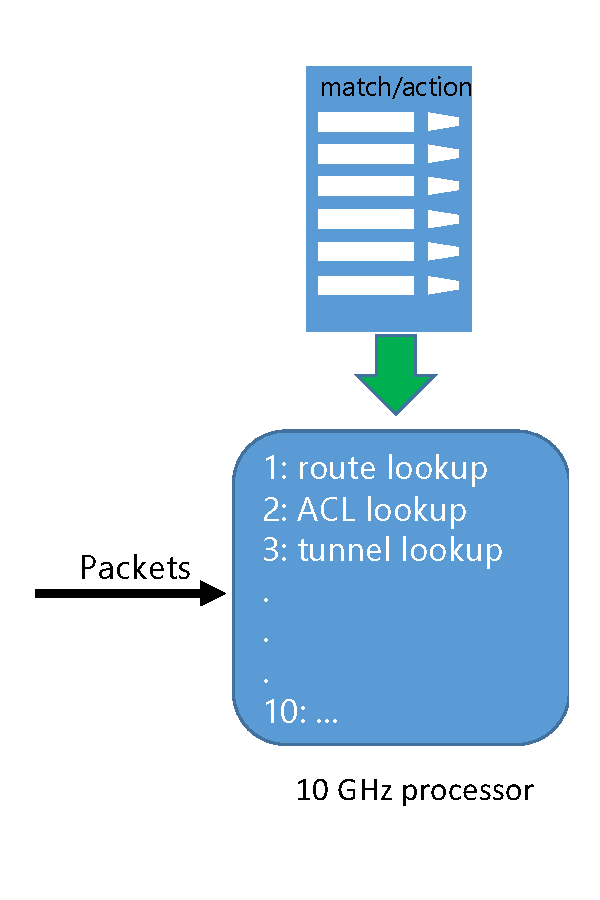
\includegraphics[width=\textwidth]{single_processor.pdf}
\caption{10 GHz processor}
\label{fig:single_processor}
\end{minipage}
\hfill
\begin{minipage}{0.7\textwidth}
\centering
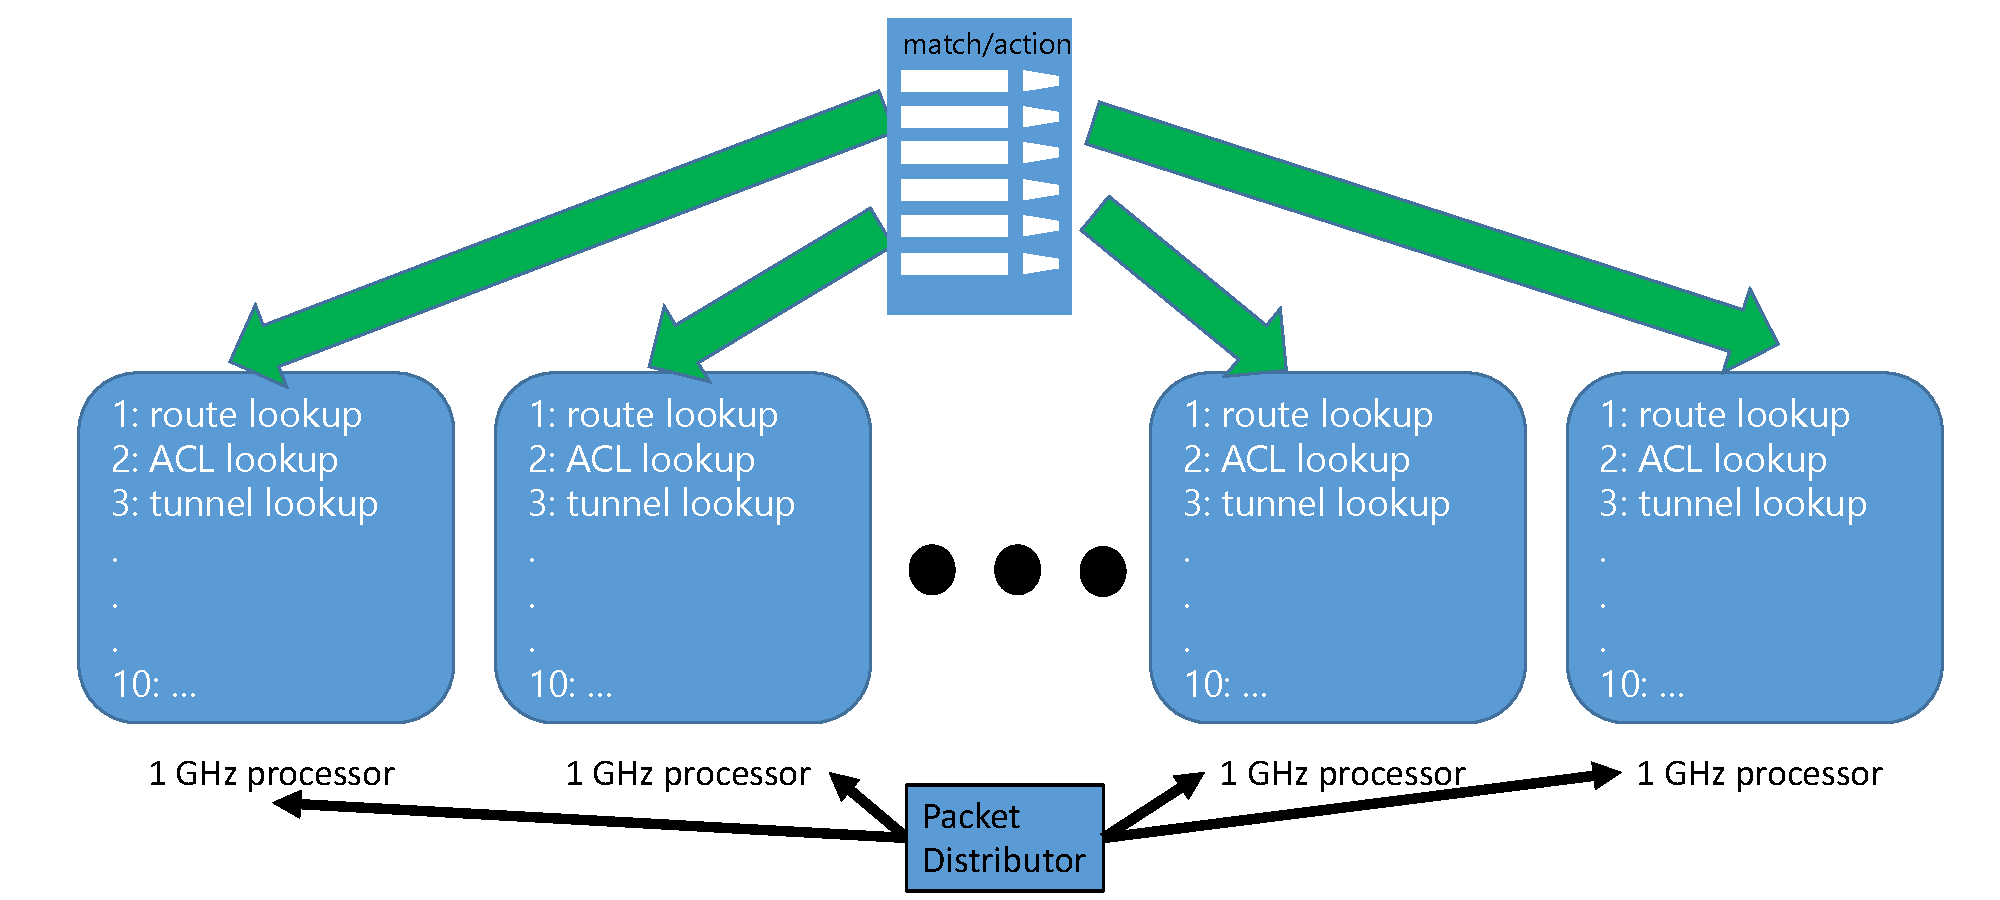
\includegraphics[width=\textwidth]{processor_array.pdf}
\caption{An array of 10 1-GHz processors. }
\label{fig:processor_array}
\end{minipage}
\caption{Two strawman designs for a high-speed router}
\end{figure}

\section{A pipeline architecture for high-speed routers}
\label{s:router_pipeline_arch}

To avoid having to use multi-ported memories, high-speed routers are typically
architected as a shared-nothing {\em pipeline}. Each pipeline stage is
dedicated to a fixed functionality, such as destination address lookup,
tuneling, measurement, or access control. Each pipeline stage has its own
dedicated local memory to store its own match-action tables, corresponding to
destination address lookup, tuneling, measurement, or access control, as the
case may be. This architecture provides parallelism: at any point, each
pipeline stage is working on a different packet. It also does so without
sharing memory between processors: each match-action table is local and can be
accessed only by the pipeline stage to which it belongs.

This pipeline architecture is the architecture followed by most high-speed
routers today. Packets arriving at a
router~(Figure~\ref{fig:detailed_pipeline}) are parsed by a parser that turns
packets into header fields. These header fields are first processed by an
ingress pipeline consisting of match-action tables arranged in stages.
Processing a packet at a stage may modify its header fields, through
match-action rules, as well as some persistent state at that stage, \eg packet
counters. After the ingress pipeline, the packet is queued. A queue might build
up any time two input ports have a packet for the same output port during the
same clock cycle. Once the scheduler dequeues the packet, it is processed by a
similar egress pipeline before it is transmitted.\footnote{In practice, the
ingress and egress pipeline can be time multiplexed on top of a single shared
physical pipeline to improve utilization~\cite{rmt}.}

\begin{figure}[!t]
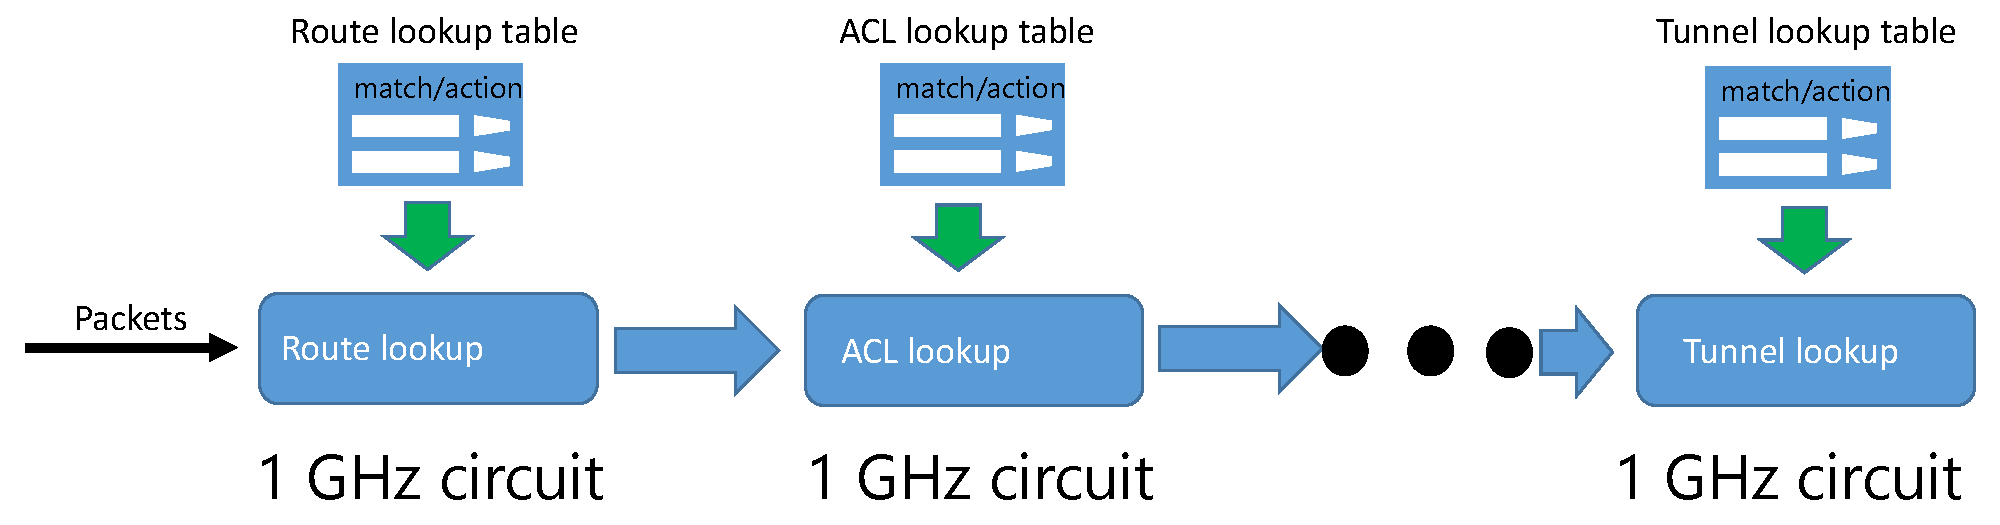
\includegraphics[width=\textwidth]{pipeline.pdf}
\caption{Pipeline architecture adopted by most high-speed routers.}
\label{fig:pipeline}
\end{figure}

\begin{figure}[!t]
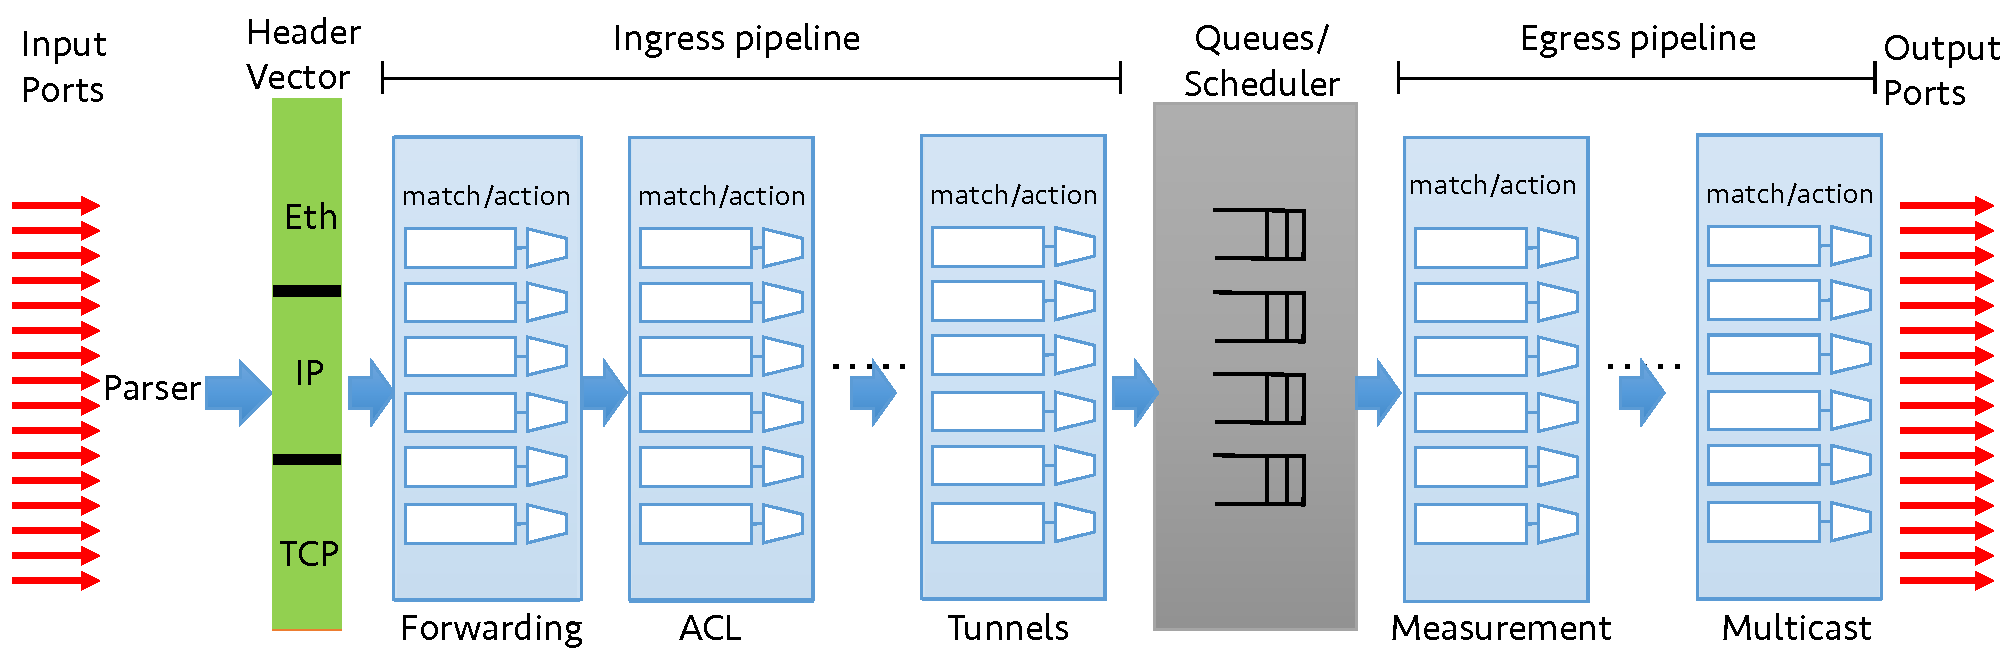
\includegraphics[width=\textwidth]{detailed_pipeline.pdf}
\caption{Architecture of a high-speed router showing the parser, pipelines, and scheduler.}
\label{fig:detailed_pipeline}
\end{figure}

\subsection{The internals of a single pipeline stage}
\label{ss:internal_pipeline_stage}
Each pipeline stage
implements the match-action model at high speed. Packets are received at a
pipeline stage at the clock rate of the pipeline (\textasciitilde1 GHz).
Within a pipeline stage, the match unit extracts the relevant packet headers
from the packets so that the extracted headers can be matched against specific
patterns in a match-action table. For instance, a match unit might extract the
TCP headers out of all the packet headers to match the TCP's source port
against 22 to detect SSH traffic and, as part of the action, prioritize SSH
traffic by setting the IP ToS field.

%TODO: rules vs. entries be consistent
Once the relevant headers are extracted, they are matched against match-action
rules stored in an on-chip match-action table. This match can either be exact
(\eg determining the next hop based on the destination's MAC address) or can
use wildcards to indicate don't-care bits (\eg matching a destination IP
address against different possible IP subnets). The memory for the match-action
table is structured as a hash table in SRAM (for exact matches) and as a
ternary content-addressable memory (TCAM) (for wildcard matches).

If a match is successful, the rule that matched against the headers of the
incoming packet is returned. This rule contains the relevant information
required for the action, such as the concrete numeric value of the output port
in the case of a destination-address lookup. If the packet does not match
successfully against any rule in the match-action table, some default action is
carried out. Typically, the default action sends the packet to the control
plane CPU of the router.

This whole processing sequence within a pipeline stage: extracting relevant
headers for a match, looking them up in a match-action table, and then carrying
out the appropriate action on a table hit or miss, can take 10s of clock
cycles for any given packet. At the same time, the pipeline stage must be ready
to accept a new packet every clock cycle. To allow this, the pipeline stage is
itself internally pipelined, \ie the header extraction for one packet proceeds
in parallel with the table lookup for a second packet and the action execution
for a third packet.

\subsection{Flexible match-action processing}
Initially the set of fields on which matches could be performed were fixed and
limited to a small set of a standard header fields (\eg TCP, UDP, and IP).
Similarly, the actions allowed on the packet headers were restricted to a fixed
set of actions, such as dropping a packet, forwarding a packet through an
output port, or setting a priority field on a packet. The common subset of
match fields and actions that were supported by most fixed-function routers was
standardized as part of the OpenFlow API~\cite{openflow}, which provided
control planes with a standardized and portable way to access the data planes
of a variety of high-speed routers.

Over time, however, the fixed nature of matches and actions led to a
progressive increase in the number of fields supported by OpenFlow~\cite{p4}.
This eventually lead to the development of flexible match-action processing as
embodied in recent high-speed routers~\cite{xpliant, flexpipe, tofino}. In
these routers, a programmable parser~\cite{gibb_parsing} allows the user to
specify a new protocol format. Using the programmable parser, the router parses
bytes into this new protocol format, and the ingress and egress pipelines can
match on header fields that are part of the new protocol format.  This is
enabled by a input multiplexer in a match-action stage, which can extract a
user-specified field from anywhere in the packet's headers for matching,
without being constrained to a fixed set of fields available at fixed locations
in the packet's headers. The net result is the ability to program a router to
recognize a new packet format, then match on fields within this new format, and
finally the ability to compose new user-defined actions out of a small set of
primitive actions that support modifications on individual packet fields.

However, flexible match-action processing largely ignores the question of
programmable manipulation of {\em state} in the data plane as part of the
action.  Instead, the primitive actions are restricted to {\em stateless}
manipulation of packet headers, \eg adding two packet headers and writing the
result into a third. As we will see in \S\ref{s:absmachine}, one of our
contributions is developing a machine model for programmable routers that
supports programmable state modification in the data plane of the router. 

\section{Using multiple pipelines to scale to higher speeds}
\label{s:router_multi_pipeline_arch}

Both the ingress and egress pipelines are shared across a number of router
ports.  They handle aggregate traffic belonging to all these ports, regardless
of packet sizes. When the aggregate traffic requirement is small enough, a
single ingress and egress pipeline suffice. For instance, a 64-port router with
a line rate of 10 Gbit/s per port and a minimum packet size of 64 bytes needs
to process around a billion packets per second, after accounting for minimum
inter-packet gaps~\cite{rmt}.  This requirement can be supported by a single
pipeline that runs at 1 GHz and is shared across all 64 ports.

For higher aggregate capacities, multiple 1-GHz pipelines are required because,
as discussed earlier, it is technically challenging to achieve a clock rate
higher than 1 GHz in most chips. While having multiple pipelines allows the
router to scale to higher aggregate speeds, it comes at the cost of fragmenting
state across different pipelines.  For instance, packets in one pipeline cannot
access state present in another pipeline. Hence, it is challenging to maintain
a piece of global state that is accessed by and modified by every packet going
through a multi-pipeline router.
%TODO: consider multi-pipeline diagram?

Even in a multi-pipeline router, there is a single shared piece of hardware for
the scheduler that enqueues packets from multiple ingress pipelines and
dequeues its packets into multiple egress pipelines. To support the ability to
handle inputs and outputs from multiple pipelines, the scheduler's memory is
multi-ported.  This is possible without considerable area overhead by
exploiting the fact that most of the scheduler's memory is structured as a set
of First In First Out Queues with a limited set of operations (\ie enqueues and
dequeues). The limited set of operations on the scheduler memory allows the
development of multi-ported memory for the scheduler without considerable area
expense.\footnote{By contrast, our strawman design for routers based on an
array of processors with shared memory (\S\ref{ss:strawman2}) requires a more
general-purpose, and hence expensive, form of multi-ported memory.}

Throughout this dissertation, we assume a single pipeline router. For
concreteness, we assume the pipeline runs at 1 GHz (\ie every pipeline stage
handles a new packet every 1 ns), although our concepts generalize to other
clock frequencies. We discuss how our ideas can be extended to multi-pipeline
routers later (\S\ref{ss:multiple_pipelines}).

\subsection{Clarifying router terminology}

Routers are classified based on several attributes in the literature. In this
subsection, we briefly discuss some of the major classifications to clarify the
terminology used in this dissertation.

At a conceptual level, routers are classified into output-queued and
input-queued routers depending on whether the queues build up at the input
ports or the output ports of a router~\cite{karol}. An output-queued router is
preferable because it offers more predictable performance: if an output port
has a large backlog of packets it only affects that output port and no other
ports.

One way to implement an output-queued router is using memory that is shared
across all output ports of the router. This memory needs to support enqueues
from any of the input ports and dequeues from any of the output ports every
clock cycle~\cite{sundar_shared_memory, dctcp}.  In addition to emulating an
output-queued router, a shared memory implementation has the benefit that the
memory pool can be allocated to output ports on demand depending on the
congestion at each output port, without committing memory to output ports at
hardware design time.

With a single ingress and a single egress pipeline shared across all ports,
sharing memory is relatively straightforward: each pipeline enqueues or
dequeues once every clock cycle, which can be supported by single-ported
memory. With multi-pipeline routers, this requires specialized multi-ported
memories in the scheduler as discussed earlier. 

Routers with single and multiple pipelines are instances of a single chip
router, where a single chip provides aggregate forwarding capacity for the full
line rate at all ports, while emulating an output-queued router. For even
higher aggregate speeds, such as those seen in core routers, multiple such
chips are put together on a motherboard in a Fat Tree topology~\cite{b4}, but
such multi-chip routers are not necessarily output-queued anymore.

Unless otherwise mentioned, a router in this dissertation refers to a
single-chip, single-pipeline, output-queued router.

\section{Summary}
This chapter provided an overview of the hardware architecture of a high-speed
router to serve as a mental model of a router chip for the rest of this
dissertation.  The programmable hardware designs that we propose are intended
to replace fixed-function router hardware within the hardware architecture
presented here.

For instance, atoms, introduced in \S\ref{ss:intro_atoms} and detailed in
\S\ref{s:absmachine}, replace fixed action units within a match-action stage.
Atoms also provide the ability to programmatically manipulate state as part of
the action.  Our hardware design for PIFOs, introduced in
\S\ref{ss:intro_pifo_hardware} and detailed in \S\ref{s:design}, replaces the
first-in first-out queues usually found in a scheduler. Finally, the on-chip
cache of our programmable key-value store, introduced in
\S\ref{ss:intro_pq_hardware} and detailed in \S\ref{sec:aggregation}, takes the
place of a match-action table within a match-action stage. The off-chip backing
store in our key-value store runs on the control plane: either on the
general-purpose CPU controlling the router or on a centralized measurement
server.
